% \documentclass[letterpaper,12pt]{article}
\documentclass{article}
\usepackage[margin=0.9in]{geometry}

\usepackage{cite}
\usepackage{listings}
\usepackage{subcaption}
\usepackage{color}
\usepackage{amsmath,amssymb}

\usepackage{graphicx}
\usepackage{float}
\usepackage{gensymb}
\usepackage{physics}
\usepackage{listings}

\usepackage[final]{hyperref} % adds hyper links inside the generated pdf file
\hypersetup{
    colorlinks=true,       % false: boxed links; true: colored links
    linkcolor=blue,          % color of internal links
    citecolor=blue,        % color of links to bibliography
    filecolor=magenta,      % color of file links
    urlcolor=blue         
}
\definecolor{dkgreen}{rgb}{0,0.6,0}
\definecolor{gray}{rgb}{0.5,0.5,0.5}
\definecolor{mauve}{rgb}{0.58,0,0.82}
\lstset{frame=tb,
  language={},
  aboveskip=1mm,
  belowskip=1mm,
  showstringspaces=false,
  columns=flexible,
  basicstyle={\small\ttfamily},
  numbers=none,
  numberstyle=\tiny\color{gray},
  keywordstyle=\color{blue},
  commentstyle=\color{dkgreen},
  stringstyle=\color{mauve},
  breaklines=true,
  breakatwhitespace=true,
  tabsize=3
}

\usepackage{titlesec}
\newcommand{\sectionbreak}{\clearpage} % start each section on a new page

\let\vec\mathbf
\def\real{\mathbb{R}}

\pdfstringdefDisableCommands{%
  \def\lstinline#1{}%
}

\begin{document}

\tableofcontents

\section{Theory}

This discussion is based on \cite{brunton2016sindy} and \cite{shea2020sindy-bvp}.
I'm going to try to outline the general case. 
\begin{align}
\vec{u} &= \vec{u}(\vec{x}, t) \\
\frac{d\vec{u}}{dt} &= \frac{d\vec{u}}{dt}(\vec{u}, \vec{x}, t)
\end{align}
for $\vec{u} \in \real^{d_u}, \,\, \vec{x} \in \real^{d_x}, \,\, t \in \real$.
The goal of SINDy is to represent $\frac{d\vec{u}}{dt}$ in a basis $B$ of size
$p$ with sparse coefficients $\vec{c} \in \real^p$.
\begin{equation}\label{eq:dudt-approx}
\frac{d\vec{u}}{dt} \approx \sum_{i=1}^p c_i \vec{b_i}(\vec{u},\vec{x},t)
\end{equation}
\begin{align}
b_i \in B = \{\vec{1}, \vec{u}, \vec{x}, t, \vec{u}^2, \vec{u}\vec{x},\vec{u}t,\vec{x}^2,\vec{x}t,t^2,\hdots,\sin\vec{u},\cos{\vec{u}}, \frac{\partial\vec{u}}{\partial \vec{x}},\hdots\}
\end{align}
This will generally be represented as a linear system with discretized $\vec{U}$
and $\vec{X}$, with the columns of the matrix $\Theta$ represented basis
functions evaluated at specific $\vec{X}$ and $t$.
\begin{equation}\label{eq:basis-system}
\frac{d\vec{U}}{dt} \approx \Theta(\vec{U}, \vec{X}, t) \vec{c}
\end{equation}

Note that when $d_x \ne 1$ or $d_u \ne 1$, the vector terms in the basis shown above
aren't mathematically well-defined, but the idea is to include polynomial terms,
and these can also include polynomial terms of separate components of the
vector, and cross terms of those components. The functions shown in the basis
above are just examples; the main idea is that the basis can have any kind of
functions of $\vec{u}$, $\vec{x}$, and $t$.

Also note that, as far as the algorithm goes, it does not matter what is on the
left-hand side. The algorithm does not take advantage of it being a time
derivative of something. It could be a time derivative (\cite{brunton2016sindy})
or a spatial derivative (\cite{shea2020sindy-bvp}), or it could just be any
variable that you want to have a sparse representation for (citation needed).
Similarly, since the basis functions can be anything, the basis matrix $\Theta$
could be a function of any variables. At its core SINDy is just sparse
regression. The following sections discuss how to set up the specific case of
having vector-valued outputs with coordinates.

\subsection{Integral formulation}

Since derivatives can give noisy data, there is an alternative integral
formulation described in \cite{schaeffer2017integral} that can be obtained by integrating
Equation~\ref{eq:dudt-approx} over time.
\begin{equation}
\vec{u}(t) - \vec{u}(0) \approx \sum_{i=1}^p c_i \int_0^t \vec{b_i}(\vec{u}(\vec{x},\tau),\vec{x},\tau) \,\, d\tau
\end{equation}
This leads to a matrix formulation in the same form as
Equation~\ref{eq:basis-system} where the basis functions are replaced with an
integral and the left-hand side is replaced by $\vec{U}(t) - \vec{U}(0)$.
The integrals can be approximated with something as simple as piecewise constant quadrature.
Assuming the input data $\vec{u}$ is collected at regularly spaced times $t_k$, the integral can be computed as:
\begin{equation}
\int_0^t \vec{b_i}(\vec{u}(\vec{x},\tau),\vec{x},\tau) \,\, d\tau \approx \Delta t \sum_{i=1}^k \vec{b_i}(\vec{u}(\vec{x},t_i),\vec{x},t_i)
\end{equation}

\subsection{Simplest dimensional case, $d_x = 0$ and $d_u = 1$} \label{section:simplest}

To get to a multi-dimensional formulation, I'll start out by describing the case when $d_x = 0$ and $d_u = 1$.
\begin{align*}
u &= u(t) \\
\frac{du}{dt} &= \frac{du}{dt}(u, t)
\end{align*}
In this case, the collected data will be a one-dimensional set of values of $u$
at different times. Let $m$ be the number of data points, and $\vec{U} \in
\real^m$ be the set of data points, where $U_k$ is the $k$-th measurement of
$u$, with a corresponding derivative $\frac{d\vec{U}}{dt}$. Let $\vec{B_i} \in
\real^m$ be the $i$-th basis function evaluated at all $m$ data points, such
that $B_{k,i}$ is the basis function evaluated at the $k$-th measurement.
Then the equation to solve is the following:
\begin{equation*}
\frac{d\vec{U}}{dt} \approx \sum_{i=1}^p c_i \vec{B_i}
\end{equation*}
This can be written as a matrix multiplication, where $\vec{B_i}$ are the
columns of $\Theta \in \real^{m \times p}$.
\begin{equation}
\frac{d\vec{U}}{dt} \approx \Theta \vec{c}
\end{equation}
This can be solved for a sparse $\vec{c}$ with a sparse least squares solver. In
this case the basis functions are functions of the two variables $u$ and $t$.

\subsection{More outputs, $d_x = 0$ and $d_u \ge 1$} \label{section:more-outputs}

When $\vec{u}$ is a vector, each measurement will have $d_u$ values. In this
case the basis functions can be made of functions of the $d_u+1$ variables
$u_1,u_2,\hdots,u_{d_u}$ and $t$. To obtain separate sparse coefficients for
each output $\frac{du_i}{dt}$, the sparse regression can be performed on each
output dimension separately. Let $\vec{U_i} \in \real^{m}$ be the measurements
for output $i$ and $\vec{c_i} \in \real^p$ be the coefficients for output $i$.
Then we can solve the equation below to find all the coefficients.
\begin{equation}\label{eq:same-theta-eqs}
\frac{d\vec{U_i}}{dt} \approx \Theta \vec{c_i} \,\,\ \text{ for $i \in \{1,2,\hdots,d_u\} $}
\end{equation}

This can be structured as a single matrix equation by letting $\vec{U_i}$ be the
columns of the matrix $\vec{U} \in \real^{m \times d_u}$, and $\vec{c_i}$ be the
columns of the matrix $\vec{c} \in \real^{p \times d_u}$. Then the equation
becomes the following:
\begin{equation*}
\frac{d\vec{U}}{dt} \approx \Theta \vec{c}
\end{equation*}
This formulation makes each output $u_i$ depend on the same set of basis
functions, stored in $\Theta$. To write it as a single matrix equation but allow
each $u_i$ to have a different set of basis functions, a block diagonal
structure can be used.

Let $\Theta^{(i)} \in \real^{m \times p_i}$ be the data for the $p_i$ basis
functions to use for output $u_i$. Let $p = \sum p_i$ be the total number of
basis functions. Then the block diagonal matrix $\Theta' \in \real^{md_u \times p}$ can be constructed
using $\Theta^{(i)}$ along the diagonal. Then flatten the data $\vec{U}$ into a
vector $\vec{U'} \in \real^{md_u}$ and flatten the coefficients $\vec{c}$ into a
vector $\vec{c}' \in \real^{p}$.
\begin{equation}\label{eq:dx0-dudt-separate-theta}
\frac{d\vec{U'}}{dt} = 
\begin{bmatrix}
\frac{d\vec{U_1}}{dt} \\ \frac{d\vec{U_2}}{dt} \\ \vdots \\ \frac{d\vec{U_{d_u}}}{dt}
\end{bmatrix}
\approx
\begin{bmatrix}
\Theta^{(1)} \\
& \Theta^{(2)} \\
& & \ddots \\
& & & \Theta^{(d_u)} \\
\end{bmatrix}
\begin{bmatrix}
\vec{c_1} \\ \vec{c_2} \\ \vdots \\ \vec{c_{d_u}}
\end{bmatrix}
= \Theta' \vec{c}'
\end{equation}
A possible problem with this formulation is that a sparse solver may enforce
sparsity on $\vec{c}$, but the desired sparsity is actually on each separate
$\vec{c_i}$. The problem is that a larger value in $\vec{c_i}$ may make the
values in $\vec{c_j}$ smaller for some $i$ and $j$. For this reason, it may be
more beneficial to use a sparse solver on the following separate equations instead:
\begin{equation}\label{eq:diff-theta-eqs}
\frac{d\vec{U_i}}{dt} \approx \Theta^{(i)} \vec{c_i} \,\,\ \text{ for $i \in \{1,2,\hdots,d_u\} $}
\end{equation}

\subsection{Handling coordinates, $d_x = 1$ and $d_u = 1$}
In this case, we have a scalar function with 1D coordinates $u = u(x,t)$. In
this case, our measurements will be snapshots of $u(x)$ at different times. Let
$n$ be the number of slices of the $x$ dimension, and $m$ be the number of
slices in the $t$ dimension. Let $\vec{U} \in \real^{m \times n}$ be the set of
data points where each column $\vec{U_j} \in \real^m = u(x_j, t)$ is the value
of $u$ at $x_j$ fixed time for each different time $t$.

This can be thought of as monitoring $n$ separate outputs similary to the case
in Section~\ref{section:more-outputs}, but additional structure can be obtained by
assuming that $u$ is governed by a PDE. In that case, $\frac{du}{dt}(u,x_j,t)$
will only depend on $x_j$, $u$, and the spatial derivatives of $u$ at $x_j$.
Thus, the linear system should be set up so that there is no dependence between
separate $x$ coordinates; each $x_j$ will have a separate basis matrix
$\Theta^{(j)}(x_j, u(x_j,t)) \in \real^{m \times p}$.

\paragraph{Varying coefficients}
This can be done in a similar manner as
Equation~\ref{eq:dx0-dudt-separate-theta}. Note that each point should use the
same set of basis functions. Let the number of basis functions at each point be
$p$. The block diagonal matrix $\Theta' \in \real^{mn \times np}$ has
$\Theta^{(j)}$ along the diagonal. Each point $x_j$ has a coefficient vector
$\vec{c_j} \in \real^p$
\begin{equation}\label{eq:coord-varying}
\frac{d\vec{U'}}{dt} = 
\begin{bmatrix}
\frac{d\vec{U_1}}{dt} \\ \frac{d\vec{U_2}}{dt} \\ \vdots \\ \frac{d\vec{U_n}}{dt}
\end{bmatrix}
\approx
\begin{bmatrix}
\Theta^{(1)} \\
& \Theta^{(2)} \\
& & \ddots \\
& & & \Theta^{(n)} \\
\end{bmatrix}
\begin{bmatrix}
\vec{c_1} \\ \vec{c_2} \\ \vdots \\ \vec{c_{n}}
\end{bmatrix}
= \Theta' \vec{c}'
\end{equation}
This formulation allows the coefficient vector to vary across space, since each
point has a separate set of basis coefficients. This formulation is used on
\cite{shea2020sindy-bvp}. An algorithm like Sequential Grouped Threshold Ridge
Regression in \cite{shea2020sindy-bvp} can be used to ensure that each $x$
coordinate uses the same sparsity for the basis functions.

\paragraph{Constant coefficients}
Alternatively, it may be desirable for the coefficients to not vary across
space; instead, a single coefficient vector should represent all points. In this
case, the input data and the matrices can be stacked so that each $x$ position
is effectively an independent data point. The matrix $\Theta' \in \real^{mn
\times p}$ can be constructed by stacking $\Theta^{(i)}$ rowwise. The
data $\vec{U}$ can be stacked into vector $\vec{U'} \in \real^{md_u}$. Each
point $x_j$ has the same coefficient vector $\vec{c} \in \real^p$

\begin{equation}\label{eq:coord-const}
\frac{d\vec{U'}}{dt} = 
\begin{bmatrix}
\frac{d\vec{U_1}}{dt} \\ \frac{d\vec{U_2}}{dt} \\ \vdots \\ \frac{d\vec{U_{n}}}{dt}
\end{bmatrix}
\approx
\begin{bmatrix}
\Theta^{(1)} \\
\Theta^{(2)} \\
\vdots \\
\Theta^{(n)} \\
\end{bmatrix}
\vec{c}
= \Theta' \vec{c}
\end{equation}

\subsection{Full multi-dimensional case, $d_x \ge 1$ and $d_u \ge 1$}
This simply combines the descriptions of the previous two sections. The $d_x$
coordinates can be linearized in some manner so that they can be referenced with
a single index $j$. Then Equation~\ref{eq:coord-varying} or~\ref{eq:coord-const}
can be used with $n$ equal to the total number of coordinate points.

Each dimension $i \in \{1,2,\hdots,d_u \}$ can be treated separately, either as
a separate column as used in Equation~\ref{eq:same-theta-eqs}
and~\ref{eq:diff-theta-eqs} or as a stack next to a block diagonal matrix as
used in Equation~\ref{eq:dx0-dudt-separate-theta}. This yields $d_u$ linear
systems so that each output dimension has its own independent set of sparse
coefficients as a solution.


\subsection{Normalization}

Consider running a sparse regression on $\dot{U} = U$ with basis functions $U$,
$100U$, and $0.01U$. The solution can be represented with either $\vec{c} =
\begin{bmatrix} 1 & 0 & 0 \end{bmatrix}$, $\begin{bmatrix} 0 & 0.01 & 0
\end{bmatrix}$, $\begin{bmatrix} 0 & 0 & 100 \end{bmatrix}$, or any result where
$c_1 + 100*c_2 + 0.01*c_3 = 1$. Note that $c_3$ has to be 100 times larger than
$c_1$ in order to have the same effect. Regularization will penalize the $c_3$
factor more than the other factors and favor the $c_2$ factor more than the
other factors, solely based on the scale of the basis functions.

Real basis function won't be scaled versions of the same function, but they will
still suffer from the same problem of larger basis columns being favored just
for having larger values. To help alleviate this problem, the input basis
functions can be normalized.

Let $D \in \real^{p \times p}$ be a diagonal matrix where each diagonal element
is the norm of the corresponding column in $\Theta$. This matrix can be
used to scale $\Theta$ to get a matrix $\Theta'$ where each column has norm 1.
\begin{equation}\label{eq:normalized-system}
\frac{d\vec{U}}{dt} \approx (\Theta D^{-1}) (D\vec{c}) = \Theta' \vec{c'}
\end{equation}
The solution of the normalized system is $\vec{c'}$, and $\vec{c}$ can be
recovered using $\vec{c} = D^{-1} \vec{c'}$.

\paragraph{TODO:} The original SINDy paper's supporting document \cite{brunton-sindy-appendix}
said that normalizing the columns of $\Theta$ may be necessary to ensure
the restricted isometry property (RIP) holds. To track down why this holds and
why this is desired, I did some citation hopping. The citation for this
statement led to a paper that made the same claim and cited another paper, and
that paper didn't seem to mention RIP or a relevant normalization, so it was a
dead end. The only document I could find supporting this RIP idea is Proposition 8 in the
blog post below, which gives the RIP constant for a matrix with normalized
columns.
\url{https://joelmoreira.wordpress.com/2014/07/31/the-restricted-isometry-property/}
TODO: figure out why a RIP matrix is good.
Hint: If a RIP matrix $A' \in \real^{m \times p}$ has a RIP constant smaller than 1,
then every submatrix $A' \in \real^{m \times k}$ must have positive eigenvalues
near 1.

\section{Examples}

\subsection{sindy\_sine}
In this example, $d_x = 0$ (no coordinates) and $d_u = 1$. There is no time dependence.
\begin{equation*}
\frac{dU}{dt} = -\sin(U) \approx -U + 0.1\overline{6}U^3 - 0.008\overline{3}U^5
\end{equation*}
The code runs the ODE from points spaced evenly around 0, with the goal of
recovering the Maclaurin series. Note that since this problem has no
coordinates, the name $x$ is used in the code instead of $U$.
\begin{lstlisting}[language={}]
                    dx/dt
 1                       0
 x             -9.9993e-01
 x*x                     0
 x*x*x          1.6626e-01
 x*x*x*x                 0
 x*x*x*x*x     -7.7962e-03
\end{lstlisting}
These values are all slightly smaller than desired. Slightly better results can
be obtained by not using regularization when doing the least squares. This can
be done with the option \lstinline{-tao_brgn_regularizer_weight 0}.
\begin{lstlisting}[language={}]
                    dx/dt
 1                       0
 x             -9.9997e-01
 x*x                     0
 x*x*x          1.6643e-01
 x*x*x*x                 0
 x*x*x*x*x     -7.9052e-03
\end{lstlisting}


\subsection{sindy\_sine\_cosine}
In this example, $d_x = 0$ (no coordinates) and $d_u = 2$. There is no time dependence.
\begin{equation*}
\frac{d\vec{U}}{dt} =
\begin{bmatrix}
-\sin(U_1) \\ \cos(U_2)
\end{bmatrix}
\approx
\begin{bmatrix}
 -U + 0.1\overline{6}U^3 - 0.008\overline{3}U^5 \\  1 - 0.5U^2 +  0.041\overline{6}U^4
\end{bmatrix}
\end{equation*}
This example effectively runs an independent ODE for each component of the vector.
The code runs the ODEs from points spaced evenly around 0, with the goal of
recovering the Maclaurin series for each term.

Note that since $\cos(x)$ is positive around 0, the ODE will evolve those values
such that they won't be centered around 0, which means the result won't be
expected to match the Maclaurin series exactly.
\begin{lstlisting}[language={}]
                                dx/dt[0]      dx/dt[1]
 1                                      0    9.9928e-01
 x[i]                         -9.9997e-01             0
 x[i]*x[i]                              0   -4.9523e-01
 x[i]*x[i]*x[i]                1.6642e-01             0
 x[i]*x[i]*x[i]*x[i]                    0    3.6669e-02
 x[i]*x[i]*x[i]*x[i]*x[i]     -7.9029e-03             0
\end{lstlisting}

In the above run, the cross term range was set to 0, so that each output
component is a function only of the corresponding input component. Without
making that constraint, noise can lead to entangled components, especially for
the non-centered cosine term. In the above runs, the data for the time
derivative was computed exactly, but in this run, a fourth-order centered finite
difference scheme is used to compute the data used for SINDy. (This was done
with the options \lstinline{-sindy_cross_term_range -1 -fd_der 1}).
\begin{lstlisting}[language={}]
                                dx/dt[0]      dx/dt[1]
 1                                      0    9.8486e-01
 x[0]                         -9.9998e-01    8.9189e-03
 x[1]                                   0    5.5136e-03
 x[0]*x[0]                              0    1.1331e-01
 x[0]*x[1]                              0   -3.0466e-02
 x[1]*x[1]                              0   -4.5908e-01
 x[0]*x[0]*x[0]                1.6643e-01   -1.3214e-01
 x[0]*x[0]*x[1]                         0   -1.6491e-02
 x[0]*x[1]*x[1]                         0   -9.6066e-03
 x[1]*x[1]*x[1]                         0   -1.6298e-02
 x[0]*x[0]*x[0]*x[0]                    0   -2.8238e-02
 x[0]*x[0]*x[0]*x[1]                    0    9.3109e-02
 x[0]*x[0]*x[1]*x[1]                    0   -1.1547e-01
 x[0]*x[1]*x[1]*x[1]                    0    2.8111e-02
 x[1]*x[1]*x[1]*x[1]                    0    1.6894e-02
 x[0]*x[0]*x[0]*x[0]*x[0]     -7.9224e-03    5.2672e-02
 x[0]*x[0]*x[0]*x[0]*x[1]               0   -4.3969e-02
 x[0]*x[0]*x[0]*x[1]*x[1]               0    3.5491e-02
 x[0]*x[0]*x[1]*x[1]*x[1]               0    5.1007e-02
 x[0]*x[1]*x[1]*x[1]*x[1]               0   -7.6728e-03
 x[1]*x[1]*x[1]*x[1]*x[1]               0    1.0493e-02
\end{lstlisting}

\subsection{sindy\_sine\_cosine\_grid}
In this example, $d_x = 2$ (2D coordinates) and $d_u = 2$. There is no time dependence.
\begin{equation*}
\frac{d\vec{U}}{dt}(x_1, x_2) =
\begin{bmatrix}
-\sin U_1(x_1,x_2) \\ \cos U_2(x_1,x_2)
\end{bmatrix}
\end{equation*}
This example effectively runs an independent ODE at each coordinate and each
component of the vector. The code runs the ODEs from points spaced evenly around
0, with the goal of recovering the Maclaurin series for each term, with the
caveat that the cosine component won't stay centered about 0.

This code essentially gives the same results as the examples above, with
enhanced problem of the regularization messing up the data. With the default
regularization parameter $10^{-4}$, the fifth order sine term is lost. Turning
it down to \lstinline{-tao_brgn_regularizer_weight 1e-7} recovers the expected
value.

An additional problem encountered here is that the the constant term in the
cosine data is lost if the left-hand side is approximated with a fourth-order
central finite difference (\lstinline{-fd_der 1}). This happens because the
finite difference doesn't approximate the first two steps or last two steps of
any run, so it zeros them out instead. This effect can be overcome by running
for more time steps so that the boundary steps have a smaller relative effect.

\subsection{sindy\_pendulum}
This example is a scalar second-order ODE, which I'll rephrase as a first-order ODE with two components.
\begin{equation*}
\frac{d^2U}{dt^2} = -\sin(U) \approx -U + 0.1\overline{6}U^3 - 0.008\overline{3}U^5
\end{equation*}
\begin{align*}
\vec{U}' &=
\begin{bmatrix}
U \\ \frac{dU}{dt}
\end{bmatrix} \\
\frac{d\vec{U}'}{dt} &=
\begin{bmatrix}
\frac{dU}{dt} \\ \frac{d^2U}{dt^2}
\end{bmatrix} =
\begin{bmatrix}
U'_2 \\ -\sin U'_1
\end{bmatrix}
\end{align*}
The code runs the ODE with initial points spaced evenly around 0, with the goal of
recovering the Maclaurin series. It performs well with 0 initial velocity.
\begin{lstlisting}[language={}]
                                    du'/dt[0]     du'/dt[1]
 1                                           0             0
 u'[0]                                       0   -9.9995e-01
 u'[1]                              1.0000e+00             0
 u'[0]*u'[0]                                 0             0
 u'[0]*u'[1]                                 0             0
 u'[1]*u'[1]                                 0             0
 u'[0]*u'[0]*u'[0]                           0    1.6633e-01
 u'[0]*u'[0]*u'[1]                           0             0
 u'[0]*u'[1]*u'[1]                           0             0
 u'[1]*u'[1]*u'[1]                           0             0
 u'[0]*u'[0]*u'[0]*u'[0]                     0             0
 u'[0]*u'[0]*u'[0]*u'[1]                     0             0
 u'[0]*u'[0]*u'[1]*u'[1]                     0             0
 u'[0]*u'[1]*u'[1]*u'[1]                     0             0
 u'[1]*u'[1]*u'[1]*u'[1]                     0             0
 u'[0]*u'[0]*u'[0]*u'[0]*u'[0]               0   -7.8459e-03
 u'[0]*u'[0]*u'[0]*u'[0]*u'[1]               0             0
 u'[0]*u'[0]*u'[0]*u'[1]*u'[1]               0             0
 u'[0]*u'[0]*u'[1]*u'[1]*u'[1]               0             0
 u'[0]*u'[1]*u'[1]*u'[1]*u'[1]               0             0
 u'[1]*u'[1]*u'[1]*u'[1]*u'[1]               0             0
\end{lstlisting}

I found that using a high initial velocity \lstinline{-v0 -2} gives bad results,
whether or not finite-differences are used to approximate $\frac{d\vec{U'}}{dt}$
(\lstinline{-fd_der}). Below is the output for \lstinline{./pendulum -v0 -2 -fd_der}.
However, this could be fixed by setting the time step size to a
smaller value with \lstinline{-dt 0.001}, which gives nearly exactly the same
results as the correct results above.
\begin{lstlisting}[language={}]
                                    du'/dt[0]     du'/dt[1]
 1                                           0             0
 u'[0]                                       0   -4.7682e+00
 u'[1]                              1.0000e+00    8.3012e+00
 u'[0]*u'[0]                                 0   -2.9006e+00
 u'[0]*u'[1]                                 0    2.7714e+00
 u'[1]*u'[1]                                 0    9.5134e+00
 u'[0]*u'[0]*u'[0]                           0   -5.2707e-01
 u'[0]*u'[0]*u'[1]                           0   -5.0834e-01
 u'[0]*u'[1]*u'[1]                           0    4.6567e+00
 u'[1]*u'[1]*u'[1]                           0    3.1919e+00
 u'[0]*u'[0]*u'[0]*u'[0]                     0   -2.7514e-02
 u'[0]*u'[0]*u'[0]*u'[1]                     0   -2.1456e-01
 u'[0]*u'[0]*u'[1]*u'[1]                     0    5.1738e-01
 u'[0]*u'[1]*u'[1]*u'[1]                     0    1.3866e+00
 u'[1]*u'[1]*u'[1]*u'[1]                     0    2.4970e-01
 u'[0]*u'[0]*u'[0]*u'[0]*u'[0]               0             0
 u'[0]*u'[0]*u'[0]*u'[0]*u'[1]               0   -1.1853e-02
 u'[0]*u'[0]*u'[0]*u'[1]*u'[1]               0             0
 u'[0]*u'[0]*u'[1]*u'[1]*u'[1]               0    1.0380e-01
 u'[0]*u'[1]*u'[1]*u'[1]*u'[1]               0    1.0797e-01
 u'[1]*u'[1]*u'[1]*u'[1]*u'[1]               0   -9.1037e-03
\end{lstlisting}

\subsection{lorenz}
In this example, $d_x = 0$ (no coordinates) and $d_u = 3$. There is no time dependence.
\begin{align*}
\frac{d\vec{U}}{dt} &=
\begin{bmatrix}
\sigma(U_2-U_1) \\
U_1(\rho-U_3)-U_2 \\
U_1U_2-\beta U_3;
\end{bmatrix} \\
\sigma &= 10,\,\, \beta = \frac{8}{3},\,\, \rho = 28
\end{align*}
This example runs in a straightforward manner and recovers the correct values
essentially exactly.
\begin{lstlisting}[language={}]
                      dx/dt[0]      dx/dt[1]      dx/dt[2]
 1                            0             0             0
 x[0]               -1.0000e+01    2.8000e+01             0
 x[1]                1.0000e+01   -1.0000e+00             0
 x[2]                         0             0   -2.6667e+00
 x[0]*x[0]                    0             0             0
 x[0]*x[1]                    0             0    1.0000e+00
 x[0]*x[2]                    0   -1.0000e+00             0
 x[1]*x[1]                    0             0             0
 x[1]*x[2]                    0             0             0
 x[2]*x[2]                    0             0             0
 x[0]*x[0]*x[0]               0             0             0
 x[0]*x[0]*x[1]               0             0             0
 x[0]*x[0]*x[2]               0             0             0
 x[0]*x[1]*x[1]               0             0             0
 x[0]*x[1]*x[2]               0             0             0
 x[0]*x[2]*x[2]               0             0             0
 x[1]*x[1]*x[1]               0             0             0
 x[1]*x[1]*x[2]               0             0             0
 x[1]*x[2]*x[2]               0             0             0
 x[2]*x[2]*x[2]               0             0             0
\end{lstlisting}


\subsection{lorenz96}
In this example, $d_x = 0$ (no coordinates) and $d_u = 36$. There is no time dependence.
\begin{align*}
\frac{dU_i}{dt} &= (U_{i+1} - U_{i-2}) U_{i-1} - U_i + F \\
F &= 8
\end{align*}
This system is very large. By default, SINDy would construct a basis that
include terms entangling each $U_i$. To make the system tractable, I set the
cross-term range to 2, so that only $U_{i-2},U_{i-1},U_i,U_{i+1},U_{i+2}$ would
be used in the basis function computation for output $\frac{dU_i}{dt}$. Below is
the output for the first three components; the rest are similar.
\begin{lstlisting}[language={}]
                     dx/dt[0]      dx/dt[1]      dx/dt[2]      dx/dt[3] 
 1                  7.8484e+00    7.8996e+00    7.8879e+00    7.8517e+00
 x[i-2]                      0             0             0             0
 x[i-1]                      0             0             0             0
 x[i]              -9.8401e-01   -9.9015e-01   -9.8526e-01   -9.8215e-01
 x[i+1]                      0             0             0             0
 x[i+2]                      0             0             0             0
 x[i-2]*x[i-2]               0             0             0             0
 x[i-2]*x[i-1]     -9.9822e-01   -9.9845e-01   -9.9859e-01   -9.9754e-01
 x[i-2]*x[i]                 0             0             0             0
 x[i-2]*x[i+1]               0             0             0             0
 x[i-2]*x[i+2]               0             0             0             0
 x[i-1]*x[i-1]               0             0             0             0
 x[i-1]*x[i]                 0             0             0             0
 x[i-1]*x[i+1]      1.0002e+00    9.9959e-01    9.9914e-01    9.9933e-01
 x[i-1]*x[i+2]               0             0             0             0
 x[i]*x[i]                   0             0             0             0
 x[i]*x[i+1]                 0             0             0             0
 x[i]*x[i+2]                 0             0             0             0
 x[i+1]*x[i+1]               0             0             0             0
 x[i+1]*x[i+2]               0             0             0             0
 x[i+2]*x[i+2]               0             0             0             0
\end{lstlisting}

\subsection{pde\_power\_grid}

In this example, $d_x = 2$ and $d_u = 1$, and there is time dependence.
\begin{align*}
\frac{dU}{dt} &= - \frac{\partial x_1}{\partial t} \frac{\partial U}{\partial x_1}
                 - \frac{\partial x_2}{\partial t} \frac{\partial U}{\partial x_2}
                 + f(t) \frac{\partial^2 U}{\partial x_2^2}
\\ \frac{\partial x_1}{\partial t} &= (x_2 - \omega_s)
\\ \frac{\partial x_2}{\partial t} &= \frac{\omega_s}{2H}(P_m - P_{max}\sin(x_1))
\\ f(t) &= \left(\frac{\lambda \omega_s}{2H}\right) ^ 2 q (1-e^{-t/\lambda})
\end{align*}
\begin{lstlisting}[language={}]
                                                    du/dt
 1                                                       0
 du/dx                                          1.0000e+00
 du/dy                                         -1.0000e-01
 d2u/dy2                                                 0
 d2u/dx2                                                 0
 t                                                       0
 (1 - exp(-t/lambda))                                    0
 x[0]                                                    0
 x[1]                                                    0
 du/dx*du/dx                                             0
 du/dx*du/dy                                             0
 du/dx*d2u/dy2                                           0
 du/dx*d2u/dx2                                           0
 du/dx*t                                                 0
 du/dx*(1 - exp(-t/lambda))                              0
 du/dx*x[0]                                              0
 du/dx*x[1]                                    -1.0000e+00
 du/dy*du/dy                                             0
 du/dy*d2u/dy2                                           0
 du/dy*d2u/dx2                                           0
 du/dy*t                                                 0
 du/dy*(1 - exp(-t/lambda))                              0
 du/dy*x[0]                                     2.1000e-01
 du/dy*x[1]                                              0
 d2u/dy2*d2u/dy2                                         0
 d2u/dy2*d2u/dx2                                         0
 d2u/dy2*t                                               0
 d2u/dy2*(1 - exp(-t/lambda))                   9.9999e-05
 d2u/dy2*x[0]                                            0
 d2u/dy2*x[1]                                            0
 d2u/dx2*d2u/dx2                                         0
 d2u/dx2*t                                               0
 d2u/dx2*(1 - exp(-t/lambda))                            0
 d2u/dx2*x[0]                                            0
 d2u/dx2*x[1]                                            0
 t*t                                                     0
 t*(1 - exp(-t/lambda))                                  0
 t*x[0]                                                  0
 t*x[1]                                                  0
 (1 - exp(-t/lambda))*(1 - exp(-t/lambda))               0
 (1 - exp(-t/lambda))*x[0]                               0
 (1 - exp(-t/lambda))*x[1]                               0
 x[0]*x[0]                                               0
 x[0]*x[1]                                               0
 x[1]*x[1]                                               0
\end{lstlisting}

\section{Performance results}

Data collected on Lorenz system by varying the number of time steps $n$ and
the number of basis functions $m$.

Building the basis matrix is linear in $n$, and grows with approximately
$m^{1.3}$.

\begin{figure}[H]
  \begin{subfigure}{\textwidth}
  \centering
  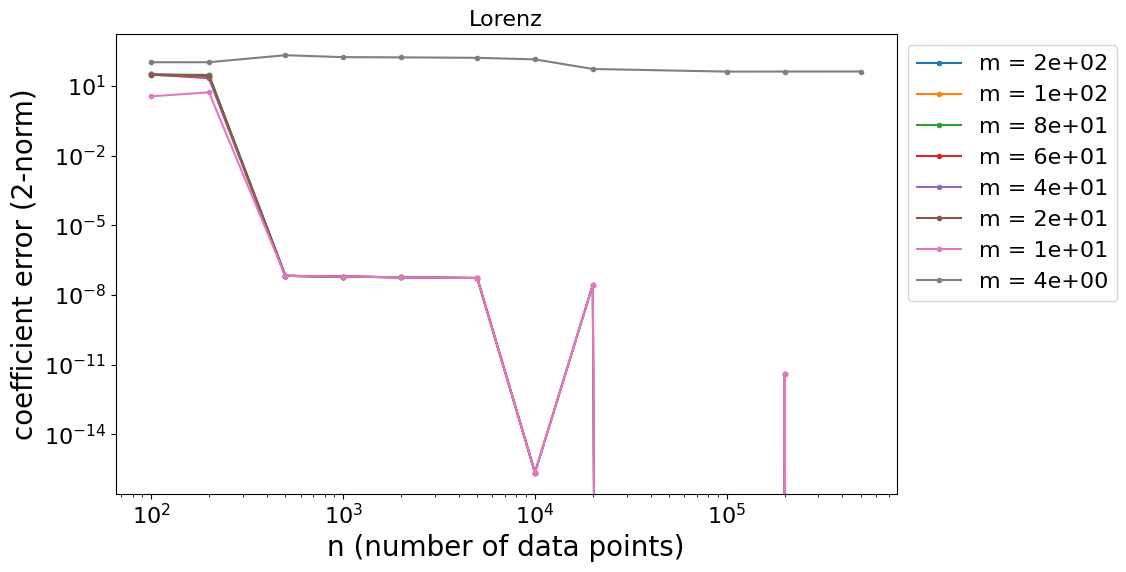
\includegraphics[width=0.8\linewidth]{sindy_plots/err_m_groups.png}
  \caption{Error grouped by $m$}
  \end{subfigure}
  \begin{subfigure}{\textwidth}
  \centering
  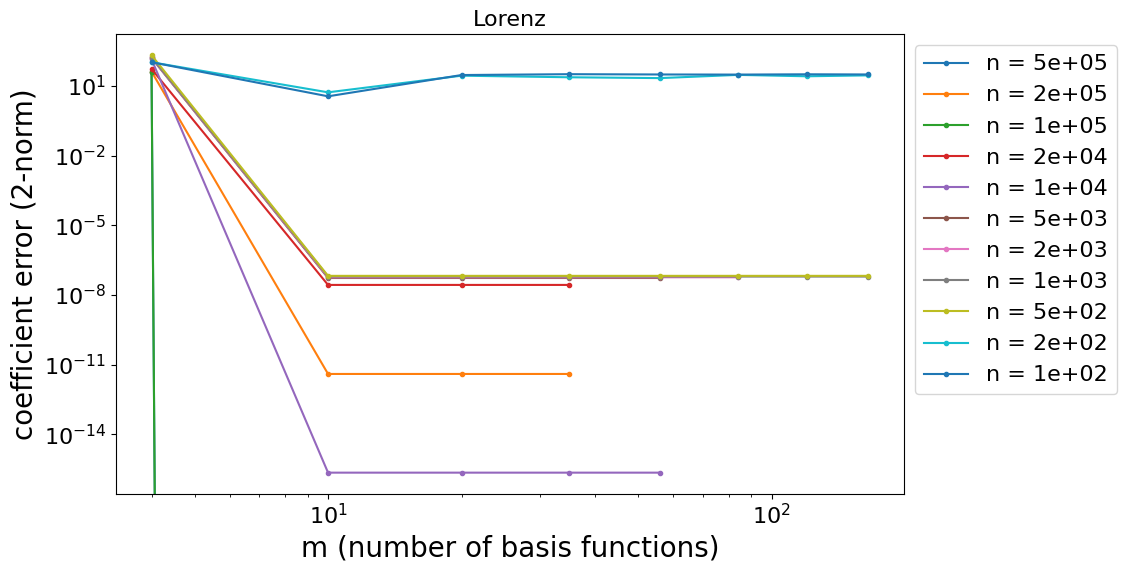
\includegraphics[width=0.8\linewidth]{sindy_plots/err_n_groups.png}
  \caption{Error grouped by $n$}
  \end{subfigure}
\caption{Timing for all the setup for the regression (including building the basis matrix)}\label{fig:lorenz-err}
\end{figure}

\begin{figure}[H]
  \begin{subfigure}{\textwidth}
  \centering
  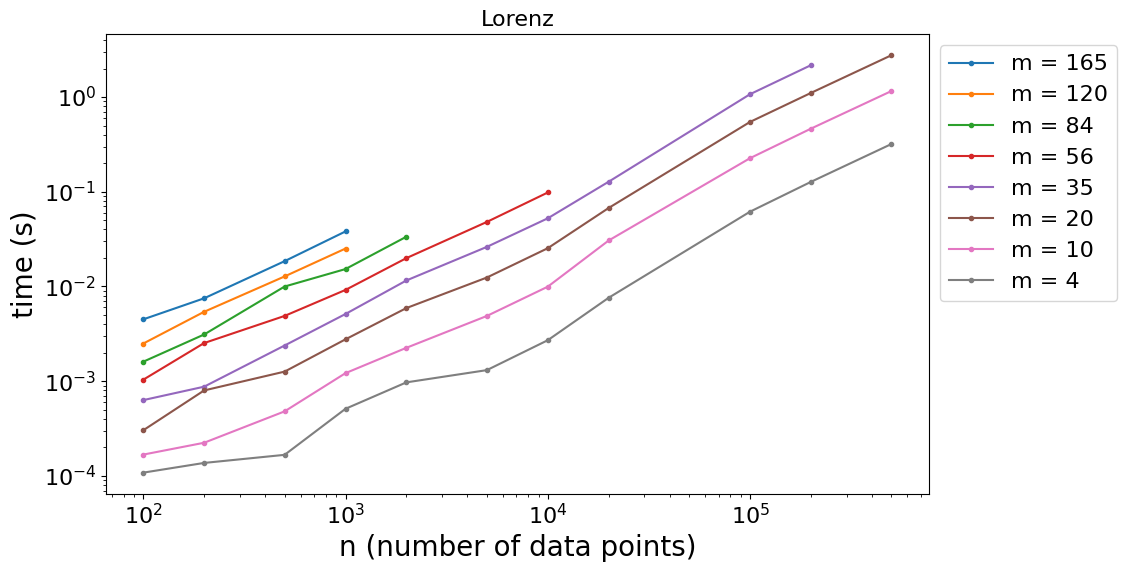
\includegraphics[width=0.8\linewidth]{setup_plots/m_groups.png}
  \caption{Runtime grouped by $m$}
  \end{subfigure}
  \begin{subfigure}{\textwidth}
  \centering
  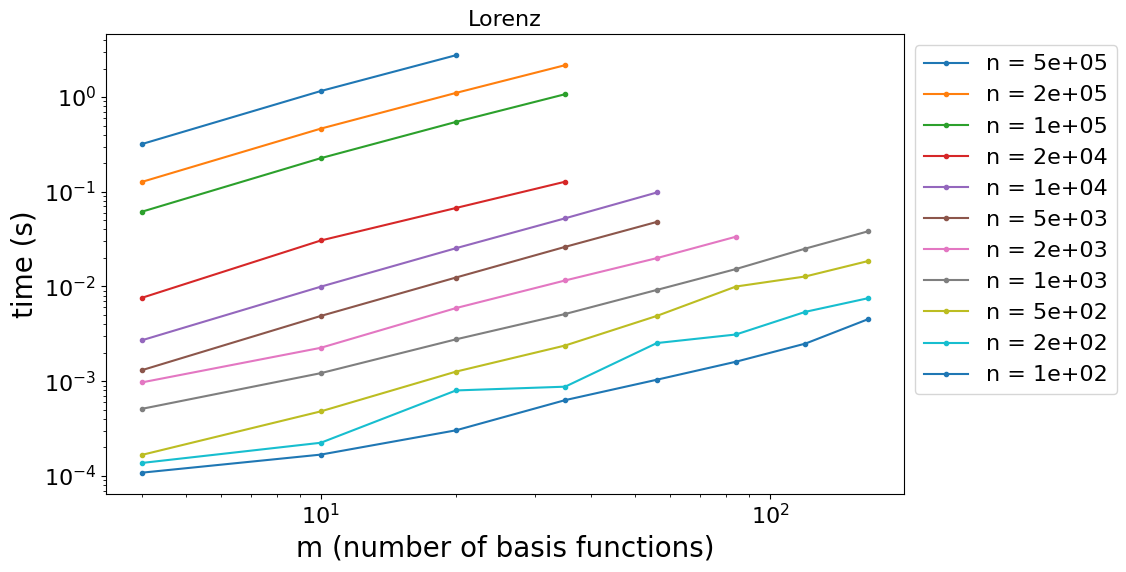
\includegraphics[width=0.8\linewidth]{setup_plots/n_groups.png}
  \caption{Runtime grouped by $n$}
  \end{subfigure}
\caption{Timing for all the setup for the regression (including building the basis matrix)}\label{fig:setup-times}
\end{figure}

\begin{figure}[H]
  \begin{subfigure}{\textwidth}
  \centering
  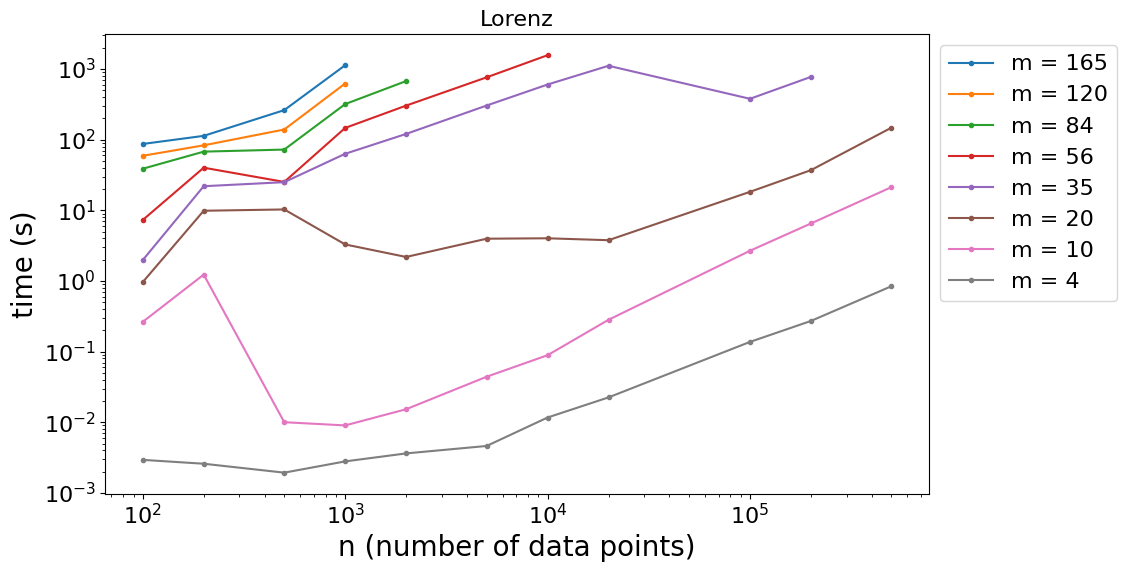
\includegraphics[width=0.8\linewidth]{sindy_plots/m_groups.png}
  \caption{Runtime grouped by $m$}
  \end{subfigure}
  \begin{subfigure}{\textwidth}
  \centering
  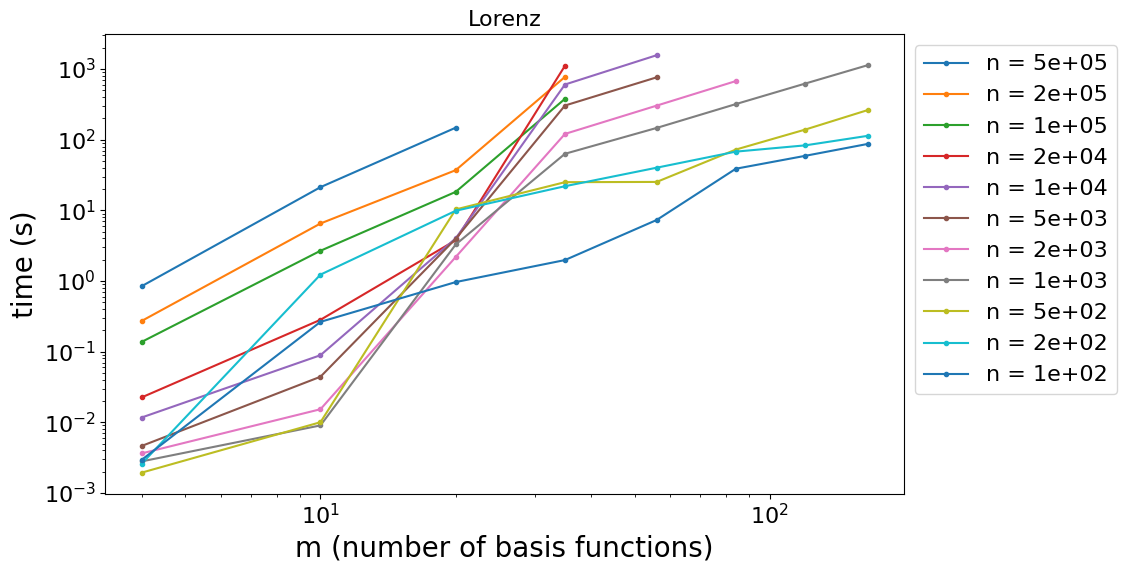
\includegraphics[width=0.8\linewidth]{sindy_plots/n_groups.png}
  \caption{Runtime grouped by $n$}
  \end{subfigure}
  \begin{subfigure}{\textwidth}
  \centering
  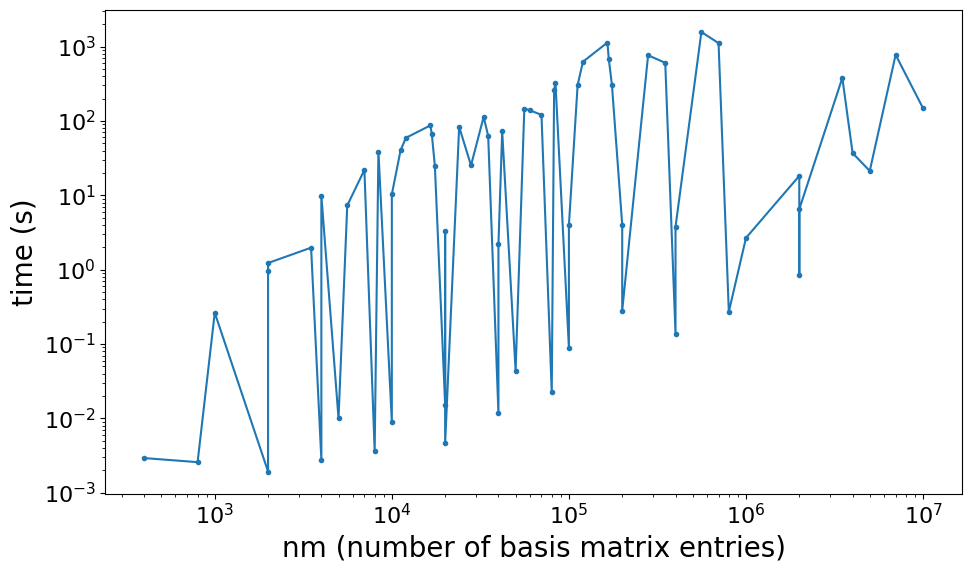
\includegraphics[width=0.64\linewidth]{sindy_plots/num_entries.png}
  \caption{Time as a function of the number of elements in the basis matrix}
  \end{subfigure}
\caption{Timing for just the regression step}\label{fig:reg-times}
\end{figure}


\section{Implementation overview}

The basis system is below (copy/pasted from Equation~\ref{eq:basis-system}).
\begin{equation}
\frac{d\vec{U}}{dt} \approx \Theta(\vec{U}, \vec{X}, t) \vec{c}
\end{equation}
An implementation requires the following steps:
\begin{enumerate}
    \item Compute the input data $\vec{U}$ (at coordinates $\vec{X}$ and times $t$). This could be data read from a file or generated with a timestepper.
    \item Compute the left-hand side $\frac{d\vec{U}}{dt}$. This can be computed with finite differences or similar methods.
    \item Compute the basis $\Theta$, which requires choosing basis functions.
    \item Compute the coefficients $\vec{c}$. This can be done with any sparse regression algorithm.
    \item Use $\vec{c}$ and the basis functions to generate $\frac{d\vec{U}}{dt}$ at the same data points or at new data points. (I have not done this yet).
\end{enumerate}

\subsection{Data generation}

I'm using PETSc's \lstinline{TS} for Step 1. I assume a fixed-time step size and
allocate memory for two arrays of \lstinline{Vec}s to hold $\vec{U}$ and
$\frac{d\vec{U}}{dt}$. Then in the TS's \lstinline{PostStep}, I record the
current value of $\vec{U}$. I have an option (in some examples) to either record
the exact value of the derivative $\frac{d\vec{U}}{dt}$ in the PostStep, or a
fourth-order central difference approximation after the run is complete.


\subsection{Basis computation}

In order for the code to work with different $d_u$ and $d_x$, the computation of
the basis needs to be flexible in how it reads the input data. The data
for a particle moving around might be stored in a 1D \lstinline{Vec} or a
\lstinline{PetscScalar} array, while the data for a PDE may be stored in a
\lstinline{Vec} with a \lstinline{DMDA}. To abstract away the data access
details, I set up a \lstinline{Variable} class. An instance of the class tracks
its data and knows how to access it properly. It also tracks its name for nice
printouts.

From the user perspective, computing the basis simply requires defining the variables
that will be present in the basis.

When the user passes these variables off to the backend, they are used to
generate the basis matrix $\Theta$.
I currently have the basis matrix set up as $d_u$ matrices as is shown in Equation~\ref{eq:diff-theta-eqs}, where
each of those matrices is constant across space, as is done in Equation~\ref{eq:coord-const}.


\subsection{Coefficient computation}

The previous step computes $\Theta$, so all this step needs to do is run a
sparse regression and return the results. I currently have Sequential
Thresholded Least Squares implemented, with parameters specified in a
\lstinline{SparseReg} class. More backends could be tested here, and we could
set sparse regression algorithm as a command-line argument.

\section{Implementation specifics}

\subsection{Cross terms}
I ran into an issue with the Lorenz 96 system in that it required polynomial
terms of degree 2, but it contains 36 independent variables. I used
Equation~\ref{eq:same-theta-eqs} to set up the system, meaning each variable
uses the same basis matrix.

The basis function generator would originally create basis functions that had
all the cross terms. In this case, that would lead to $\binom{36 + 2}{2} = 703$
basis functions. Then the algorithm takes forever to run. In this case, we know
that only nearby terms will affect each other, so I added a
\lstinline{cross_term_range} parameter, which I'll call $c$. For output DOF $i$,
it will only include input DOFs $i-c,i-c+1,\hdots,i,\hdots,i+c$. So there will
be a total of $d = 2*c+1$ terms included. For $c=2$ reduces the number of basis
functions from 703 to $\binom{d+2}{2} = \binom{7}{2} = 21$, which is much more
manageable. Since each output DOF has a different set up of basis functions,
this required changing from Equation~\ref{eq:same-theta-eqs} to
Equation~\ref{eq:diff-theta-eqs} to maintain a separate basis matrix for each
output DOF.

This setup also helps the sine-cosine example. By setting the cross term range
to 0, there is no intermingling of $U_1$ and $U_2$ in the basis functions.

For examples with coordinates ($d_x \ne 0$), the cross term range currently only
applies to DOFs within a point. I.e., for a point's output DOF $i$, it will only
include input DOFs $i-c,i-c+1,\hdots,i,\hdots,i+c$ at that point.

\subsection{Basis matrix generation}

\lstinline{SINDyBasisAddVariables} sets up the basis matrices. There is a
separate matrix for each output DOF, so there are $d_u$ matrices to build.
Each matrix is built by looping through each basis function, and for each basis function,
looping through each output coordinate and adding all $m$ outputs to the for that coordinate.
This iteration procedure generates $\Theta'$ from Equation~\ref{eq:coord-const} column-wise.

\section{Things to do}

\subsection{Speed}
\begin{itemize}
    \item Get it working in parallel.
\end{itemize}

\subsection{Basis functionality}
\begin{itemize}
    \item Make it possible to use the computed coefficients to get the
      $\frac{d\vec{U}}{dt}$ approximation at a specific point or sets of points.
      A good way to do this may be to restructure the basis to make it easy to
      apply to a dataset and get back the computated basis values as some data
      structure that can then be multiplied with the computed coefficients.
    \begin{itemize}
        \item Perhaps the \lstinline{Variable} can have a function pointer that knows
          how to compute itself given the inputs, and then the basis computation can
          return the computed basis functions as \lstinline{Variable} objects. The
          basis function type can take an array of \lstinline{Variable} objects.
        \item The inputs to the basis function may have a prescribed order of
          computation, so I may need to track a directed acyclic graph to do the
          computation correctly. E.g., for the power grid example, the nominal
          inputs would be $\vec{U}$, $\vec{X}$, and $t$, but the current example
          computes the $\sin(X_1)$ and $1-e^{-t/\lambda}$ terms first. Then
          those terms are given to the cross-term calculating function to build
          up the polynomials terms. I could rely on the user to compute their
          custom terms themselves, but it'd be more user-friendly to do it
          automatically.
    \end{itemize}
\end{itemize}

\subsection{Data interface}
\begin{itemize}
    \item Handle bad data points better. Perhaps supporting an interface to
      specify which points to not include in the linear system. (Current bad
      effects: the system has erroneous data that will mess up the regression.
      In the first case below, this will simply make the constant term more
      likely to be 0, and in the second case below, it may mess up all the
      results.)
    \begin{itemize}
        \item For example, when doing a fourth-order centered finite difference
          to estimate $\frac{du}{dt}$, the first two points and last two points
          don't have an estimate. I have been setting them to 0, but it would be
          good to support ignoring specific input data points.
        \item For example, on Dirichlet boundaries, $\frac{du}{dt} = 0$ no
          matter what the PDE equations are, so those points should be thrown
          out. This is different from the above problem because the above
          problem throws out a whole \lstinline{Vec}, while this requires
          throwing out specific values within a \lstinline{Vec}.
    \end{itemize}
\end{itemize}

\subsection{Sparse regression}

\begin{itemize}
    \item Handle threshold selection better.
    \begin{itemize}
        \item It would be good to be able to specify different thresholds for
          different degrees of freedom.
        \item It would be good to be to have automated methods for picking a
          threshold. E.g., something like Section 3.3 in
          \cite{shea2020sindy-bvp}, which uses a loss similar to AIC.
        \item In the supplemental information for \cite{rudy2017sindy-pde}, an
          automated threshold-selecting algorithm incrementally increases or
          decreases the threshold depending on the change in the
          $\ell_0$-regularized error.
    \end{itemize}

    \item Do non-regularized least squares after thresholding is complete? This
      will make the selected non-zero coefficients better match the data.

    \item Is there a way to do normalization better? One problem is that the
      current column scaling means coefficients get bigger and bigger as more
      data is added, which means the threshold parameter and regularization
      factor need to be changed accordingly. 
    \begin{itemize}
        \item The original SINDy paper (in the supporting information document)
          normalizes in order for the restricted isometry property to hold
          \cite{brunton2016sindy}, but I don't know why that's desirable.
        \item A SINDy PDE paper uses $\ell_\infty$ normalization
          \cite{schaeffer2017sindy-pde2}. With this method, adding more data
          will make the coefficients bigger only if the extra data has larger
          values than the existing data.
    \end{itemize}

    \item Add ADMM as an option to do the regularized least squares? I think the
      sparse regression step in SINDy should call a backend that can be swapped
      out for various least squares algorithms.
\end{itemize}

\subsection{Derivatives}

\begin{itemize}
    \item \cite{schaeffer2017sindy-pde2} computes spatial derivatives with the spectral method.
\end{itemize}

\subsection{File I/O}

\begin{itemize}
    \item Add support to write a computed basis to a file and read it from a
      file. This will let different sparse regularization strategies be tested
      without regenerating the data.
\end{itemize}

\subsection{Integrals}

Support for the integral formulation may be useful. Supporting both the integral
and the derivative formulations within the same framework would make it easier
to empirically compare them. It might also be interesting to combine them. I.e.,
create a combined derivative/integral system (by concatenating the data points
from each method) to see if better coefficients are obtained.
\begin{equation*}
\begin{bmatrix}
\frac{d\vec{U}}{dt} \\ \vec{U} - \vec{U}_0
\end{bmatrix}
\approx
\begin{bmatrix}
\Theta(\vec{U}, \vec{X}, t) \\ \int_0^t \Theta(\vec{U}, \vec{X}, \tau) \,\, d\tau
\end{bmatrix}
\vec{c}
\end{equation*}

\bibliographystyle{unsrt}
\bibliography{sources}


\section{Appendix}

\subsection{Non-polynomial extraction}

The inclusion of many non-polynomial basis functions can inflate the basis
matrix $\Theta$ to be too large. We would like to be able to use only polynomial
basis functions and then post-process the results to extract the non-polynomial
terms based on some polynomial expansion (e.g., Taylor series) of those terms.

\paragraph{Note:} This section discusses a completely different problem compared to the other
sections in this document, so the notation used here is completely independent
of the other sections.


\subsubsection{Subtracting out non-polynomial functions}

Let $f_j(x) = \sum_{i=0}^\infty A_{ij} x^i$ be a polynomial series representing a function,
and let $f_j^{(d)} = \sum_{i=0}^d A_{ij} x^i$ be the degree $d$ truncation of
the series. Let $g(y) = \sum_{i=0}^d b_i y^i$ be the known function that we want
to extract non-polynomial terms from. We want to express $g(y)$ in terms of
functions $f_i(x)$, where $y$ may be a scaled version of $x$.
\begin{align*}
g(y) = \sum_{i=0}^d k_i y^i + \sum_{j=1}^n c_j f_j^{(d)}(\sigma_j y)
\end{align*}
We'd like to determine $c_i$ and $\sigma_j$. The $k_i$ is used to absorb all the
polynomials factors that aren't represented by the sum of the non-polynomial
functions. The equation can be separated into $d+1$ equations by treating each
$y^j$ coefficient independently.
\begin{align*}
\sum_{i=0}^d b_i y^i &= \sum_{i=0}^d k_i y^i + \sum_{i=0}^d \sum_{j=1}^n A_{ij} c_j \sigma_j^i y^i
\\ \implies b_i &= k_i + \sum_{j=1}^n A_{ij} c_j \sigma_j^i
\,\,\,\,\, \text{ for $i \in \{0, \hdots, d\}$}
\end{align*}
This is a nonlinear problem due to the $\sigma_j^i$ term. I'll define $A_{ij}' = A_{ij} \sigma^i_j$,
\begin{align*}
\vec{b} &= \vec{k} + \vec{A}'(\vec{\sigma}) \vec{c}
\end{align*}
We want sparsity in $\vec{k}$ and $\vec{c}$, which we can maybe approximate with
the $\ell_1$ norm.
\begin{align*}
&\min_{\vec{c},\vec{\sigma}} ||\vec{k}||_1 + ||\vec{c}||_1
\\& \text{subject to } \vec{k} =  \vec{b} - \vec{A}'(\vec{\sigma})\vec{c}
\end{align*}
Or equivalently,
\begin{align*}
\min_{\vec{c},\vec{\sigma}} ||\vec{b} - \vec{A}'(\vec{\sigma})\vec{c}||_1 + ||\vec{c}||_1
\end{align*}
Running this sparse optimization will show the active non-polynomial terms in
$\vec{c}$, although I'm not sure what a good way to run this optimization would
be.

\paragraph{SINDy application:} Run SINDy with just polynomials and then use the
above strategy to determine what non-polynomial terms are present. The
coefficients for those terms can be computed as done above, or those terms can
be added to the SINDy library for SINDy to be run again with the correct
non-polynomial terms.

Perhaps it could be combined in the SINDy optimization, with $\vec{k}$
representing the polynomial terms and $\vec{c}$ representing the non-polynomial
terms.
\begin{align*}
\min_{\vec{k},\vec{c},\vec{\sigma}} & ||\vec{k}||_1 + ||\vec{c}||_1
\\\text{subject to } \vec{k} &=  \vec{b} - \vec{A}'(\vec{\sigma})\vec{c}
\\ & \vec{b} = \arg \min_{\vec{b}'} ||\Theta \vec{b}' - \tfrac{d\vec{U}}{dt}||_2^2 + \lambda ||\vec{b}'||_1
\end{align*}

\paragraph{Simplification:} It will make the problem easier if the $\sigma_j$
are assumed to be 1. Then the system becomes linear.
\begin{align*}
&\min_{\vec{c}} ||\vec{k}||_1 + ||\vec{c}||_1
\\& \text{subject to } \vec{k} =  \vec{b} - \vec{A}\vec{c}
\end{align*}
Or equivalently,
\begin{align*}
&\min_{\vec{c}} \left|\left|
\begin{bmatrix} \vec{b} \\ 0 \end{bmatrix}
-
\begin{bmatrix} \vec{A} \\ \vec{I}_n \end{bmatrix}
\vec{c}
\right|\right|_1
\end{align*}
where $\vec{I}_n$ is the identity.
In this case, we can think of this optimization as simply expressing the
original coefficients $\vec{b} \in \real^d $ in a new basis $\vec{B} \in
\real^{d \times (n+d)}$, which is composed of the original polynomial basis,
plus extra functions. Then we want to find the set of coefficients $\vec{c}' \in
\real^(d+n)$, such that $\vec{b} = \vec{B} \vec{c'}$ and $\vec{c'}$ is as sparse
as possible. Using the notation from above, the variables are defined as follows,
\begin{align*}
\vec{c}' &= \begin{bmatrix} \vec{k} \\ \vec{c} \end{bmatrix} \\
\vec{B} &= \begin{bmatrix} \vec{I}_d & \vec{A} \end{bmatrix}
\end{align*}
\subsubsection{Factoring out non-polynomial functions}

The above formulation handles cases where $g(y)$ is equal to a polynomial plus
some non-polynomial terms, where the non-polynomial terms have to be specified
in advance (e.g., sine, cosine, the exponential function). But there may be
terms like $x \sin(x)$ or $x\sin x + x^3\sin x$, where a polynomial is
multiplied by a non-polynomial. These could be included as basis functions, but
if we can extract them automatically, it will make the basis library more
tractable. Consider a function that is multiplied by a monomial of degree $r \le
d_r$. (The previous section is equivalent to $d_r=0$. This section essentially
augments the non-polynomial library with the product of polynomials with the
non-polynomials).
\begin{align*}
x^r f_j(x) = \sum_{i=0}^\infty A_{ij} x^{r+i} = \sum_{i=r}^\infty A_{i-r,j} x^{i}
\end{align*}


Again, let $g(y) = \sum_{i=0}^d b_i y^i$ be the known function that we want
to extract non-polynomial terms from. We want to express $g(y)$ in terms of
functions $f_i(x)$ multiplied by monomials.
\begin{align*}
g(y) &= \sum_{i=0}^d k_i y^i + \sum_{j=1}^n \sum_{r=0}^{d_r} c_{jr} y^r f_j^{(d)}(\sigma_j y)
\\   &= \sum_{i=0}^d k_i y^i + \sum_{j=1}^n \sum_{r=0}^{d_r} c_{jr} \sigma_j^{-r} x^r f_j^{(d)}(\sigma_j y)
\end{align*}
\begin{align*}
\sum_{i=0}^d b_i y^i &= \sum_{i=0}^d k_i y^i + \sum_{j=1}^n \sum_{r=0}^{d_r} \sum_{i=r}^d A_{i-r,j} c_{jr} \sigma_j^{i-r} y^i \\
\sum_{i=0}^d b_i y^i &= \sum_{i=0}^d k_i y^i + \sum_{j=1}^n \sum_{i=0}^d \sum_{r=1}^{\min(i,d_r)} A_{i-r,j} c_{jr} \sigma_j^{i-r} y^i
\\ \implies b_i &= k_i + \sum_{j=1}^n \sum_{r=1}^{\min(i,d_r)}  A_{i-r,j} \sigma_j^{i-r} c_{jr}
\,\,\,\,\, \text{ for $i \in \{0, \hdots, d\}$}
\end{align*}
Linearize $c_{jr}$ by treating $jr$ as a single index that goes from 1 to $nd_r$,
and let the matrix $\vec{A}' \in \real^{d \times nd_r}$ be defined as $A_{i,jr}' =
A_{i-r,j}\sigma_j^{i-r}$. This yields the same form as the previous section.
\begin{align*}
\vec{b} &= \vec{k} + \vec{A}'(\vec{\sigma}) \vec{c}
\end{align*}
We want sparsity in $\vec{k}$ and $\vec{c}$, which we can maybe approximate with
the $\ell_1$ norm, although this optimization may not work.
\begin{align*}
&\min_{\vec{c},\vec{\sigma}} ||\vec{k}||_1 + ||\vec{c}||_1
\\& \text{subject to } \vec{k} =  \vec{b} - \vec{A}'(\vec{\sigma})\vec{c}
\end{align*}

\subsection{One at a time}

The optimization problem above may be too difficult. An alternative method is to
extract one non-polynomial function at a time. This can be repeated for any
desired non-polynomial function.

Again, let $g(y) = \sum_{i=0}^d b_i y^i$ be the known function that we want to
extract non-polynomial terms from. We want to express $g(y)$ in terms of
functions $f(x)$ multiplied by monomials, plus a polynomial function $h$.
Assume we have a truncated series expansion of $f$ in terms of polynomials.
\begin{align*}
g(y) &= h(y) + c f^{(d)}(\sigma y) \\
\sum_{i=0}^d b_i y^i &= \sum_{i=0}^d k_i y^i + \sum_{i=0}^d c a_i \sigma^i x^i
\\ \implies b_i &= k_i + c a_i \sigma^i 
\\ \implies \vec{b} &= \vec{k} + c D(\sigma) \vec{a} 
\\ D(\sigma) &= \text{diag}(1, \sigma, \sigma^2, \ldots, \sigma^d)
\end{align*}
We want to choose $c$ and $\sigma$ such that they zero out at least one term in $\vec{k}$.
Since we're choosing two parameters, though, we'll be able to zero out two terms.
A direct algorithm would do the following:
\begin{enumerate}
  \item For any two entries $i,j$ in $\vec{k}$, with $i < j$:
  \begin{enumerate}
    \item Skip this $i,j$ pair if $a_i a_j b_i b_j = 0$, which means  one of the
      terms doesn't show up in $g$, so zeroing this term out leads to $c = 0$,
      or it means one of the terms doesn't show up in $f$, so we can't use it
      zero out terms in $g$.
    \item Solve for $c$ and $\sigma$ to make these two entries 0.
      \begin{equation*}
        \sigma = \left(\frac{a_i b_j}{a_j b_i} \right)^{\frac{1}{j-i}} \text{ and } c = \frac{b_i}{a_i\sigma^i}
      \end{equation*}
    \item Record a measure of the sparsity of $\vec{k}$.
  \end{enumerate}
  \item Choose the $c$ and $\sigma$ that lead to the best sparsity of $\vec{k}$,
  or choose them to be zero if the sparsity of $\vec{b}$ is better.
\end{enumerate}
One this function is extracted, the algorithm can be repeated for a different
function. Determining the optimal extractions for a library of non-polynomial
functions may be a combinatorially large problem.

\end{document}